В ходе работы над рефератом я выполнил следующие задачи:
 
\begin{enumerate}
    \item дал определение компьютерного вируса и рассмотрел историю их появления;
    \item изучил классификацию вирусов по различным признакам: среде обитания, способу заражения, деструктивным возможностям и особенностям алгоритма;
    \item разобрал механизмы работы вирусов на примере загрузочного вируса;
    \item рассмотрел основные признаки проявления вирусного заражения;
    \item изучил основные типы антивирусных программ (детекторы, доктора, ревизоры, фильтры, вакцины) и провёл обзор современных антивирусных решений.
\end{enumerate}
 
\begin{figure}[h]
    \centering
    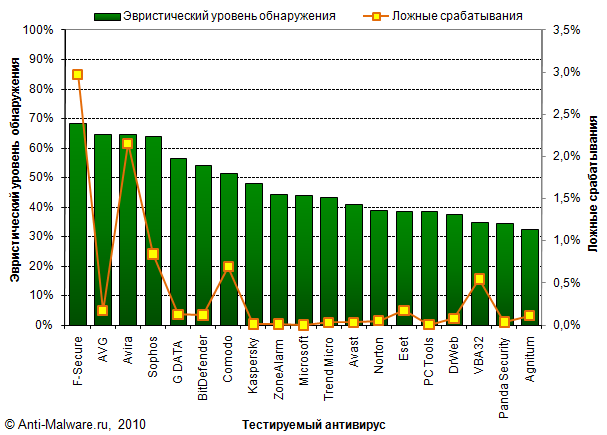
\includegraphics[width=0.6\textwidth]{images/antivirus_comparison.png}
    \caption{Сравнение эффективности антивирусных программ}
    \label{fig:antivirus_comparison}
\end{figure}
 
Несмотря на широкую распространённость антивирусных программ, вирусы продолжают «плодиться». Чтобы справиться с ними, необходимо создавать более универсальные и качественно новые антивирусные программы, которые будут включать в себя все положительные качества своих предшественников.
 
К сожалению, на данный момент нет такой антивирусной программы, которая гарантировала бы защиту от всех разновидностей вирусов на 100\%, но некоторые фирмы, например «Лаборатория Касперского», на сегодняшний день достигли неплохих результатов.
 
Защищённость от вирусов зависит и от грамотности пользователя. Применение вкупе всех видов защит позволит достигнуть высокой безопасности компьютера и, соответственно, информации.